\documentclass{article}

\usepackage[utf8x]{inputenc}
\usepackage[T1]{fontenc}
\usepackage[francais]{babel}
\usepackage{xcolor}
\usepackage{listings}
\usepackage{mathptmx}
\usepackage{anyfontsize}
\usepackage{t1enc}
\usepackage[top=2cm, bottom=2cm, left=2cm, right=2cm]{geometry}
\usepackage{titlesec}
\usepackage{titling}
\usepackage[linesnumbered, french, frenchkw, onelanguage]{algorithm2e}
\usepackage{graphicx}
\usepackage{enumitem}
\usepackage[colorlinks = true,
            linkcolor = black,
            urlcolor  = black,
            citecolor = black,
            anchorcolor = black]{hyperref}

\newcommand{\changeurlcolor}[1]{\hypersetup{urlcolor=#1}}

\renewcommand\maketitlehooka{\null\mbox{}\vfill}
\renewcommand\maketitlehookd{\vfill\null}

\definecolor{codegreen}{rgb}{0,0.6,0}
\definecolor{codegray}{rgb}{0.5,0.5,0.5}
\definecolor{codepurple}{rgb}{0.58,0,0.82}
\definecolor{backcolour}{rgb}{0.95,0.95,0.92}
\definecolor{codekeywords}{rgb}{0.1,0.53,0.92}

\lstdefinestyle{c++}{
    backgroundcolor=\color{backcolour},   
    commentstyle=\color{codegreen},
    keywordstyle=\color{codekeywords},
    numberstyle=\tiny\color{codegray},
    stringstyle=\color{codepurple},
    basicstyle=\ttfamily\footnotesize,
    breakatwhitespace=false,         
    breaklines=true,                 
    captionpos=b,                    
    keepspaces=true,                 
    numbers=left,                    
    numbersep=5pt,                  
    showspaces=false,                
    showstringspaces=false,
    showtabs=false,                  
    tabsize=2,
    texcl=true,
    inputencoding=utf8,
    extendedchars=true,
    literate=
  {á}{{\'a}}1 {é}{{\'e}}1 {í}{{\'i}}1 {ó}{{\'o}}1 {ú}{{\'u}}1
  {Á}{{\'A}}1 {É}{{\'E}}1 {Í}{{\'I}}1 {Ó}{{\'O}}1 {Ú}{{\'U}}1
  {à}{{\`a}}1 {è}{{\`e}}1 {ì}{{\`i}}1 {ò}{{\`o}}1 {ù}{{\`u}}1
  {À}{{\`A}}1 {È}{{\'E}}1 {Ì}{{\`I}}1 {Ò}{{\`O}}1 {Ù}{{\`U}}1
  {ä}{{\"a}}1 {ë}{{\"e}}1 {ï}{{\"i}}1 {ö}{{\"o}}1 {ü}{{\"u}}1
  {Ä}{{\"A}}1 {Ë}{{\"E}}1 {Ï}{{\"I}}1 {Ö}{{\"O}}1 {Ü}{{\"U}}1
  {â}{{\^a}}1 {ê}{{\^e}}1 {î}{{\^i}}1 {ô}{{\^o}}1 {û}{{\^u}}1
  {Â}{{\^A}}1 {Ê}{{\^E}}1 {Î}{{\^I}}1 {Ô}{{\^O}}1 {Û}{{\^U}}1
  {œ}{{\oe}}1 {Œ}{{\OE}}1 {æ}{{\ae}}1 {Æ}{{\AE}}1 {ß}{{\ss}}1
  {ç}{{\c c}}1 {Ç}{{\c C}}1 {ø}{{\o}}1 {å}{{\r a}}1 {Å}{{\r A}}1
  {€}{{\EUR}}1 {£}{{\pounds}}1,
}
\lstset{style=c++}


\title{Outils d'aide à la décision TP3\\Job Shop}
\author{Arquillière Mathieu - Zangla Jérémy}
%\date{\today}
%\date{\vspace{-5ex}}
\date{}

\begin{document}

\begin{titlepage}
  \maketitle
\end{titlepage}

\tableofcontents
\newpage
\listoffigures
\listofalgorithms
\newpage

\section{Optimisation d'un Job Shop}

\subsection{Evaluation d'un graphe}
On cherche ici à optimiser un problème de Job Shop.
C'est un problème composé de $n$ jobs, chacun ayant une séquence
sur $m$ machines. Par exemple prenons un problème à 3 jobs et 3 machines
avec les séquences suivantes:
$$
P_1 : (m_1, 10) \rightarrow (m_2, 4) \rightarrow (m_3, 25)
$$
$$
P_2 : (m_1, 15) \rightarrow (m_3, 16) \rightarrow (m_2, 12)
$$
$$
P_3 : (m_3, 11) \rightarrow (m_1, 12) \rightarrow (m_2, 21)
$$
On modélise un Job Shop sous la forme d'un graphe. Celui-ci possède
$n \times m$ sommets ($n$ représentant le nombre de jobs et $m$
le nombre de machines).

\begin{figure}[!ht]
  \caption{Représentation sous forme de graphe d'un Job Shop}
  \label{Graphe exemple}
  \centering
  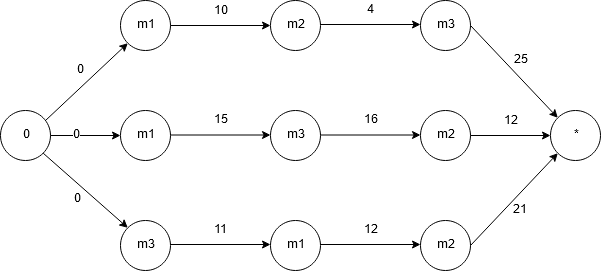
\includegraphics[scale=0.5]{images/OAD_grapheJS.png}
\end{figure}

Pour obtenir une solution au problème, on
utilise un vecteur de Bierwirth. En parcourant ce vecteur, on
peut identifier les opérations correspondant à chaque élément
et déduire la machine associé.

\begin{figure}[!ht]
  \caption{Exemple de vecteur de Bierwirth}
  \label{Vecteur de Bierwirth}
  \centering
  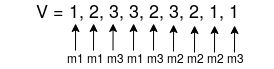
\includegraphics[scale=0.75]{images/OAD_vecteur_bierwirth.png}
\end{figure}

Cela permet de donner un ordre dans lequel sont exécutées les
tâches. A partir de ça, on trouve les arcs disjonctifs entre les
sommets du graphe et on obtient un graphe disjonctif.

\begin{figure}[!ht]
  \caption{Graphe disjonctif du Job Shop}
  \label{Graphe disjonctif}
  \centering
  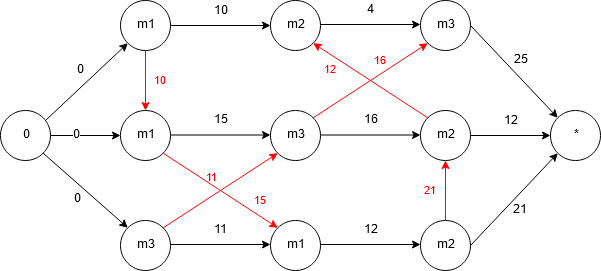
\includegraphics[scale=0.5]{images/OAD_grapheJS_disonctif.png}
\end{figure}

\newpage

Enfin on effectue un algorithme de plus court chemin pour obtenir les \emph{starting times}
de chaque tâche.

\begin{figure}[!ht]
  \caption{Graphe disjonctif du Job Shop avec les \emph{starting times}}
  \label{Graphe disjonctif avec starting times}
  \centering
  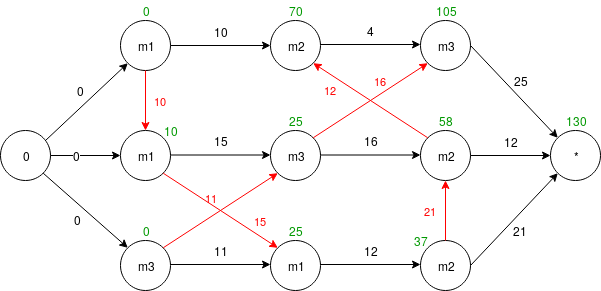
\includegraphics[scale=0.5]{images/OAD_grapheJS_disjonctif_pcc.png}
\end{figure}

Pour créer l'algorithme correspondant à ces étapes, il faut d'abord définir
les structures de données dont on aura besoin.
\begin{itemize}[label=$\bullet$]
  \item \emph{St} : un tableau de taille $n\times m$ pour contenir les \emph{starting times}
  \item \emph{pred} : un tableau de taille $n\times m$ pour contenir les précédents
  \item \emph{P'} : un tableau de taille $n\times m$ contenant les "poids", les temps d'exécution de chaque tâche
  \item \emph{U'} : un tableau de taille $n\times m$ contenant les séquences de chaque job
  \item \emph{N} : un tableau de taille $m$ contenant le nombre de fois qu'on trouve la machine $i \in 1,...,m$ pour trouver le prédecesseur
  \item \emph{MP} : un tableau de taille $m$ contenant la tâche passée en dernier sur la machine $i \in 1,...,m$
\end{itemize}

\vspace{0.25cm}
On a ensuite l'algorithme \emph{évaluer} permettant d'obtenir les \emph{starting times} et les prédecesseurs à
partir d'un vecteur de Bierwirth.

\begin{algorithm}[H]
    \For{$i=0$ \KwTo $N$}
    {
      j = V[i]\;
      N[j] = N[j] + 1\;
      pos = T[j][N[j]]\;
      \If{$N[j] > 1$}
      {
        prec = pos - 1\;
        \If{$St[prec] + P'[prec] > St[pos]$}
        {
          St[pos] = St[prec] + P'[prec]\;
          Pred[pos] = prec\;
        }
      }
      machine = U'[pos]\;
      \If{$MP[machine] != 0$}
      {
        prec = MP[machine]\;
        \If{$St[prec] + P'[prec] > St[pos]$}
        {
          St[pos] = St[prec] + P'[prec]\;
          Pred[pos] = prec\;
        }
      }
      MP[machine] = pos\;
    }
    \caption{Algorithme évaluer}
\end{algorithm}

\newpage
\subsection{Recherche Locale}
Dans cette partie l'objectif est d'améliorer une solution. Pour cela, on effectuera des
changements sur le chemin critique d'une solution existante. On parcourt en partant de la
fin le chemin critique et lorsque deux tâches qui se suivent sur ce chemin sont sur la
même machine, on tente d'inverser les deux éléments correspondants dans le vecteur de
bierwirth et de recalculer une nouvelle solution, qu'on garde si elle s'est améliorée.
Pour éviter que cet algorithme ne se finisse pas, on intègre un nombre maximum d'itérations
à ne pas dépasser, dans notre cas \emph{iter\_max} est de 15.

\vspace{0.25cm}
\begin{algorithm}[H]
  i = NT\;
  j = pred[i]\;
  \While{$j \neq 0$ et $iteration < iter\_max$}
  {
    \eIf{$U'[j] == U'[i]$}
    {
      Calculer position de i et j\;
      V' = V\;
      tmp = V'[$pos_i$]\;
      V'[$pos_i$] = V'[$pos_j$]\;
      V'[$pos_j$] = tmp\;
      evaluer(S')\;
      \eIf{S' est meilleur que S}
      {
        S = S'\;
        V = V'\;
        i = NT\;
        j = pred[i]\;
      }{
        i = j\;
        j = pred[j]\;
      }
    }{
      i = j\;
      j = pred[j]\;
    }
  }
  \caption{Algorithme de recherche locale}
\end{algorithm}

\subsection{GRASP (Greedy Randomized Adaptive Search Procedure)}
Cet algorithme (toujours visant à optimiser au maximum la solution trouvée) itere un certain
nombre de fois la méthode de chercher 5 "voisins" d'une solution donnée et on garde la meilleure pour
la prochaine itération. On obtient les voisins en échangeant des éléments du vecteur de Bierwirth, 
dans notre implémentation, la recherche de voisins boucle tant que l'on a pas trouvé
5 voisins différents et pas déjà utilisé (afin de ne pas bloquer l'algorithme,
on itere cela un nombre maximum de fois, en l'occurence 25).
De la même façon que la recherche locale, on met en place un maximum d'iterations
(100 dans notre implémentation).

\vspace{0.25cm}
\begin{algorithm}[H]
  \For{$i = 1$ \KwTo $iter\_max$}
  {
    Choisir au hasard $V$ \emph{(vecteur de Bierwirth)}\;
    Avec de vecteur on obtient une solution $S$\;
    \While{on n'a pas obtenu 5 voisins différents}
    {
      $V = generer\_un\_voisin(S)$\;
      $\rightarrow$ permutation de 2 éléments dans le vecteur\;
      $\rightarrow$ evaluer et recherche locale\;
      Tester le voisin avec la table de hash\;
    }
    $nS$ : nouvelle solution $\rightarrow$ meilleur des 5 voisins\;
  }
  \caption{Algorithme GRASP}
\end{algorithm}

\newpage
Pour savoir si les voisins trouvés sont bien différents et que l'on a pas déjà trouvé cette
solution, on utilise une table de hachage. Cela consiste à trouver un identifiant unique
(ou presque) à chaque solution et d'avoir un tableau indicé avec ces identifiants qui permet
de savoir si la solution a déjà été trouvée ou non.

Formule de hachage:
$$
h(S) = \sum_{i = 0}^n (St_i)^2 \% k
$$
\emph{n} : nombre de sommets du graphe de la solution\\
\emph{k} : taille du tableau de hash (suffisament grand).

\section{Résultats}

On utilise les instances de la \href{http://people.brunel.ac.uk/~mastjjb/jeb/orlib/files/jobshop1.txt}{OR-Library}
afin de réaliser nos tests.

\subsection{Evaluer}

\begin{figure}[!ht]
\caption{Résultats de notre implémentation de \emph{evaluer} avec LA01.txt}
\begin{lstlisting}[language=c++]
Nombre de machines : 5
Nombre de pièces : 10
Temps total : 1069
Vecteur : ( 4 7 8 6 4 6 7 3 10 2 3 8 1 10 4 7 1 7 3 7 9 9 10 10 9 9 9 4 4 6 6 1 8 6 10 3 8 2 2 3 2 2 1 5 5 8 1 5 5 5 )
Prédécesseurs :  ( 26 37 28  7  4 17 39  7  8  9 31 46 12 19 50 -1 16 12 45 19 15  4 22 23 24 16 26 43 28 20 -1 31  1 33 34 -1  6 49 30  8 47 13 42 43 44 32 46 34 42 29 )
Starting times : ( 131 213 516 860 915 132 808 860 876 902 69 223 321 645 704  0 77 321 579 645 716 915 949 1013 1032 77 131 437 516 722  0 69 152 239 326  0 153 487 784 876 302 363 412 437 481 146 223 326 412 608 )
Chemin limitant (ordre inverse) : 25 <- 24 <- 23 <- 22 <- 4 <- 7 <- 39 <- 30 <- 20 <- 19 <- 45 <- 44 <- 43 <- 42 <- 13 <- 12 <- 46 <- 32 <- 31
\end{lstlisting}
\end{figure}

\subsection{Evaluer puis recherche locale}

\begin{figure}[!ht]
\caption{Résultats de notre implémentation de \emph{recherche locale} avec LA01.txt}
\begin{lstlisting}[language=c++]
Nombre de machines : 5
Nombre de pièces : 10
Temps total : 1032
Vecteur : ( 4 7 8 6 4 6 7 3 10 2 3 8 1 10 4 7 1 7 3 7 9 9 10 10 9 9 9 4 6 6 6 1 8 4 10 3 8 2 2 3 2 2 1 5 5 8 1 5 5 5 )
Prédécesseurs :  ( 26 37 28  7  4 17 39  7  8  9 31 46 12 19 50 -1 16 12 45 30 15  4 22 23 24 16 26 43 28 29 -1 31  1 33 34 -1  6 49 20  8 47 13 42 43 44 32 46 34 42 29 )
Starting times : ( 131 213 516 823 878 132 771 823 839 865 69 223 321 645 704  0 77 321 579 670 716 878 912 976 995 77 131 437 516 608  0 69 152 239 326  0 153 487 747 839 302 363 412 437 481 146 223 326 412 608 )
Chemin limitant (ordre inverse) : 25 <- 24 <- 23 <- 22 <- 4 <- 7 <- 39 <- 20 <- 30 <- 29 <- 28 <- 43 <- 42 <- 13 <- 12 <- 46 <- 32 <- 31
\end{lstlisting}
\end{figure}

\newpage
\subsection{GRASP}
Pour tester \emph{GRASP}, on l'exécute 20 fois sur chaque instance.

\begin{center}
  \begin{tabular}{ | c | c | }
    \hline
    Instance de Job-Shop & Temps moyen (ms) \\
    \hline
    \hline
    LA01.txt & 14.0759 \\ \hline
    LA02.txt & 12.2875 \\ \hline
    LA03.txt & 11.7334 \\ \hline
    LA04.txt & 12.4472 \\ \hline
    LA05.txt & 14.5207 \\ \hline
    LA06.txt & 15.2889 \\ \hline
    LA07.txt & 15.0473 \\ \hline
    LA08.txt & 15.1696 \\ \hline
    LA09.txt & 15.6707 \\ \hline
    LA10.txt & 15.0829 \\ \hline
    LA11.txt & 18.7042 \\ \hline
    LA12.txt & 18.5126 \\ \hline
    LA13.txt & 18.678 \\ \hline
    LA14.txt & 18.2111 \\ \hline
    LA15.txt & 18.6646 \\ \hline
    LA16.txt & 14.1486 \\ \hline
    LA17.txt & 13.5904 \\ \hline
    LA18.txt & 14.5861 \\ \hline
    LA19.txt & 13.0146 \\ \hline
    LA20.txt & 13.8519 \\ \hline
  \end{tabular}
\end{center}

\end{document}
